\documentclass[13pt]{beamer}

\usepackage{Handle}



\newcommand{\Title}{Title }
\newcommand{\Subtitle}{Subtitle}
\newcommand{\Institute}{Institute Name}
\newcommand{\InstituteAddress}{Institute Address}
\newcommand{\SubmittedBy}{Submitted By}
\newcommand{\SubmittedTo}{Submitted To}
\newcommand{\ImageUrl}{Images/graph.jpg}




\subject{DAA}

\small
\date{\today}




\begin{document}
	\begin{frame}[noframenumbering,plain,t]

		\begin{tikzpicture}[remember picture, overlay]
			\node[opacity = 0.8] at (current page.center)
			{
				
\includegraphics[height = 1.5\paperwidth]{Images/bg4.png}
			};
		\end{tikzpicture}

		\MakeTitle

	\end{frame}


	\begin{frame}{Outline }
		\begin{tikzpicture}[remember picture, overlay]
			\node[opacity = 0.2] at (current page.center)
			{
				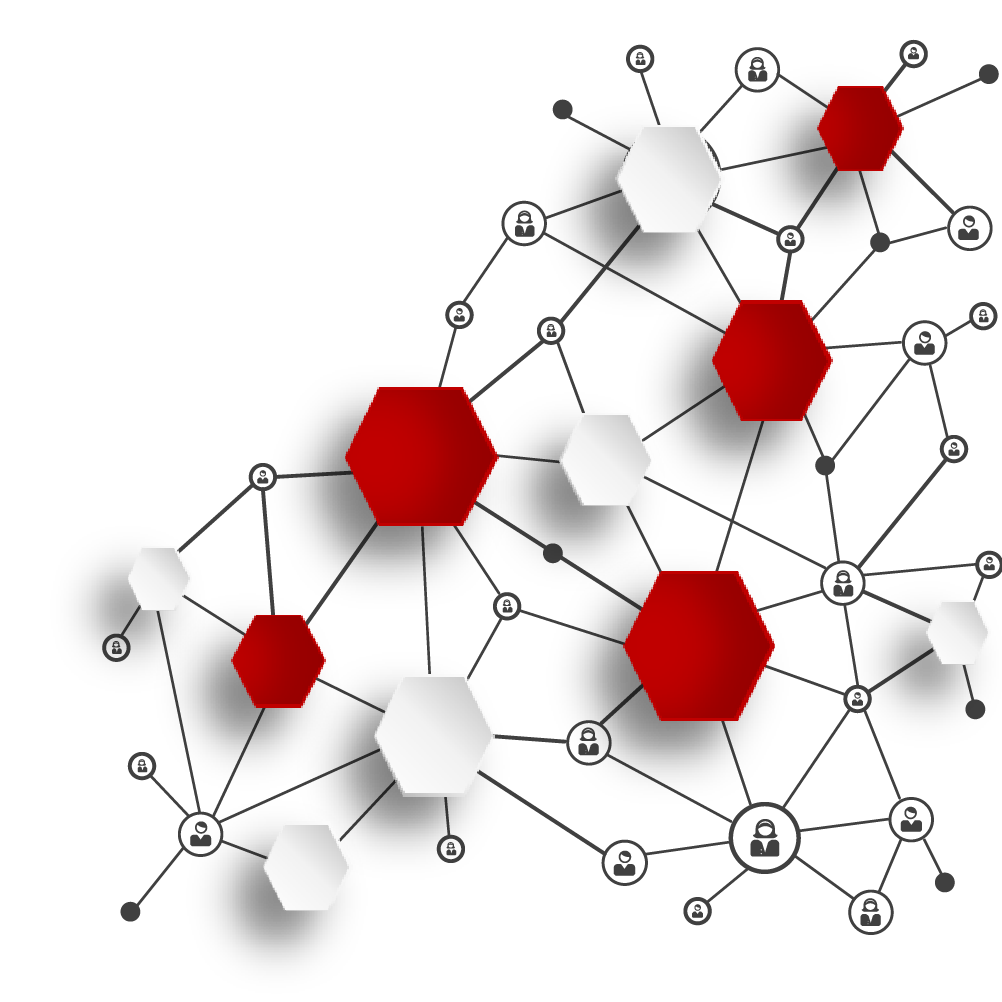
\includegraphics[height = 0.75\paperwidth]{Images/bg3.png}
			};
		\end{tikzpicture}

		\normalsize
		\tableofcontents
	\end{frame}


	\section{Intro}
	   \setbeamercolor{section in head/foot}{bg=arsenic,fg=white}
	\setbeamercolor{frametitle}{bg=airforceblue,fg=white}
	\setbeamercolor{author in head/foot}{bg=arsenic,fg=white}

	\begin{frame}[t,allowframebreaks]{Introduction to Graphs}

		\begin{itemize}
			\item  A Graph is a non-linear data structure consisting of vertices and edges.
			\item The \textbf{Vertices} are sometimes also referred to as nodes and the \textbf{Edges} are lines or arcs that connect any two nodes in the graph.

			\begin{bee}[More formally]{white}{arsenic}
				A Graph is composed of a set of vertices V and a set of edges E. \\
				The graph is denoted by \textbf{G(V,E)}.
			\end{bee}

			\item Graph data structures are a powerful tool for representing and analyzing complex relationships between objects or entities.
			\item They are particularly useful in fields such as social network analysis, recommendation systems, and computer networks.
			\item In the field of sports data science, graph data structures can be used to analyze and understand the dynamics of team performance and player interactions on the field.

		\end{itemize}

	\end{frame}


	\section{Types of Graph}

	\setbeamercolor{section in head/foot}{bg=cyan,fg=black}
	\setbeamercolor{frametitle}{bg=aqua,fg=black}
	\setbeamercolor{author in head/foot}{bg=aqua,fg=black}

	\begin{frame}[t,allowframebreaks]{Types of Graph}
		\begin{columns}
			\column{0.5\textwidth}
			\begin{bee}[Undirected Graph,width = 6cm]{black}{aqua}
				A graph in which edges do not have any direction.
			\end{bee}
			\column{0.55\textwidth}
			\begin{Rbee}[Directed Graph,width = 6cm]{arsenic}{aqua}
				A graph in which edge has direction.
			\end{Rbee}
		\end{columns}
		\begin{figure}
			\centering
			\href{https://media.geeksforgeeks.org/wp-content/uploads/20200630114438/directed.jpg}{
				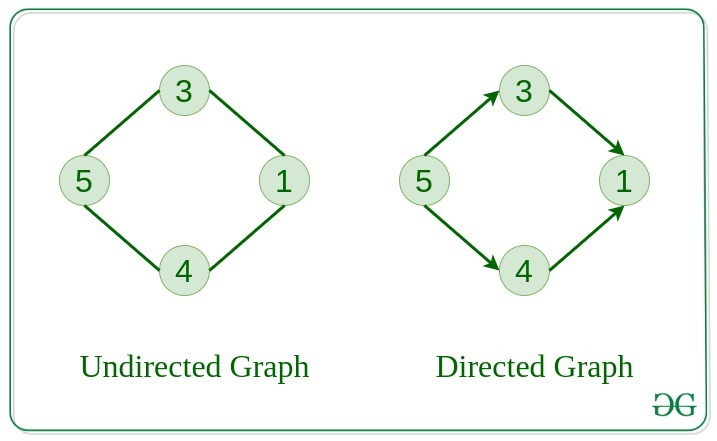
\includegraphics[height =0.37\paperheight]{Images/directed.png}
			}
		\end{figure}


		\begin{bee}[Complete Graph,width = 8cm]{white}{deepmagenta}
			A graph in which every pair of distinct nodes is connected by an edge
		\end{bee}

		\begin{Rbee}[Forest,width = 0.9\paperwidth]{white}{arsenic}
			A collection of trees or disjoint tree-like structures within a graph
		\end{Rbee}
		\begin{bee}[Tree,width = 0.9\paperwidth]{white}{blue}
			A special case of an acyclic graph in which there is a single root node, and every other node is connected by exactly one edge.
		\end{bee}






	\end{frame}

\end{document}